% NeurReps / NeurIPS 2026 workshop format: 61 cm x 85 cm, portrait.
% Custom LaTeX poster; dimensions from official PosterInstructions (2026-11-02).
\documentclass{article}
\usepackage[paperwidth=61cm,paperheight=85cm,margin=0cm]{geometry}
\usepackage[T1]{fontenc}
\usepackage{lmodern}
\usepackage{amsmath,amssymb,graphicx,tikz,xcolor,qrcode}
\usepackage[hidelinks]{hyperref}
\renewcommand{\familydefault}{\sfdefault}
\pagestyle{empty}
\definecolor{ink}{HTML}{172D40}
\definecolor{teal}{HTML}{007D80}
\definecolor{pale}{HTML}{EAF5F3}
\definecolor{muted}{HTML}{4A5E69}
\definecolor{rulecolor}{HTML}{C7D8DB}
\newcommand{\bodyfont}{\fontsize{23}{30}\selectfont}
\newcommand{\smallfont}{\fontsize{21}{27}\selectfont}
\newcommand{\heading}[1]{{\color{teal}\fontsize{28}{33}\selectfont\bfseries #1}\par\vspace{.4cm}}
\newcommand{\place}[4]{\node[anchor=north west,inner sep=0pt,text width=#3cm,align=left] at (#1,-#2) {#4};}
\setlength{\parindent}{0pt}
\setlength{\parskip}{.35cm}
\hypersetup{pdftitle={Determinants of hyperparameter robustness in connectome reservoir computing},pdfauthor={Miles Walter Churchland and collaborators}}
\DeclareMathSizes{23}{23}{16}{12}
\DeclareMathSizes{21}{21}{15}{11}
\begin{document}
\null
\begin{tikzpicture}[remember picture,overlay,x=1cm,y=1cm]
\begin{scope}[shift={(current page.north west)}]
\fill[ink] (0,0) rectangle (61,-12.3);
\fill[teal] (0,-12.3) rectangle (61,-12.55);
\place{2}{1.25}{57}{{\color{white}\fontsize{17}{21}\selectfont\bfseries NeurReps 2026\hfill Symmetry and Geometry in Neural Representations}}
\place{2}{3}{57}{{\color{white}\fontsize{54}{62}\selectfont\bfseries Determinants of hyperparameter robustness\par in connectome reservoir computing}}
\place{2}{8.65}{57}{{\color{white}\fontsize{22}{28}\selectfont Miles Walter Churchland\textsuperscript{1}, Raul de Palma Aristides\textsuperscript{2}, Jordi Garcia-Ojalvo\textsuperscript{1},\par Anna Ritz\textsuperscript{3}, Greg Anderson\textsuperscript{4}, Miguel C. Soriano\textsuperscript{2}}}
\place{53.1}{4.0}{5.3}{{\color{white}\fontsize{15}{18}\selectfont\bfseries FULL PAPER}\par\vspace{.15cm}\href{https://arxiv.org/abs/2609.07355}{\begingroup\setlength{\fboxsep}{5mm}\colorbox{white}{\qrcode[height=3.4cm]{https://arxiv.org/abs/2609.07355}}\endgroup}\par\vspace{.1cm}{\color{white}\fontsize{13}{16}\selectfont arXiv:2609.07355}}
\place{2}{10.75}{57}{{\color{white}\fontsize{17}{21}\selectfont \textsuperscript{1}Universitat Pompeu Fabra\quad \textsuperscript{2}IFISC, CSIC--UIB\quad \textsuperscript{3}Biology, Reed College\quad \textsuperscript{4}Computer Science, Reed College}}

\fill[pale] (2,-13.4) rectangle (59,-20.0);
\place{2.8}{13.85}{32.4}{{\color{teal}\fontsize{16}{20}\selectfont\bfseries RESEARCH QUESTION}\par\vspace{.1cm}{\color{ink}\fontsize{27}{32}\selectfont\bfseries Which reservoir features support robust computation?}\par\vspace{.15cm}{\color{ink}\fontsize{21}{27}\selectfont Reservoir performance can vary with hyperparameters. We compare the structured \textit{C.~elegans} connectome with controlled network variants to test which architectures remain stable across 96 settings.}}
\place{2.8}{18.1}{32.4}{{\color{ink}\fontsize{18}{22}\selectfont\bfseries Higher performance accompanies greater sensitivity; normalization also changes with excitatory/inhibitory (E/I) edge balance.}}
% The diagram is a conceptual pipeline; it is not a measurement.
\draw[rulecolor,line width=1pt] (36,-14.2) -- (36,-19.3);
\node[draw=teal,fill=white,rounded corners=3pt,minimum width=4.2cm,minimum height=1.5cm,align=center,text=ink,font=\fontsize{17}{21}\selectfont] at (39.1,-16.0) {Input\\signal};
\node[draw=teal,fill=white,rounded corners=3pt,minimum width=5.5cm,minimum height=1.5cm,align=center,text=ink,font=\fontsize{17}{21}\selectfont] at (46.6,-16.0) {Recurrent\\reservoir};
\node[draw=teal,fill=white,rounded corners=3pt,minimum width=4.4cm,minimum height=1.5cm,align=center,text=ink,font=\fontsize{17}{21}\selectfont] at (54.8,-16.0) {Linear\\readout};
\draw[-latex,teal,line width=1.5pt] (41.4,-16) -- (43.7,-16);
\draw[-latex,teal,line width=1.5pt] (49.5,-16) -- (52.4,-16);
\place{43.7}{17.15}{6}{{\color{muted}\fontsize{16}{19}\selectfont Fixed network}}
\place{52.8}{17.15}{5}{{\color{muted}\fontsize{16}{19}\selectfont Trained}}
\place{37}{18.3}{21}{{\color{ink}\fontsize{16}{20}\selectfont Inputs drive nonlinear dynamics; only the readout is fitted.}}


\place{2}{20.8}{17.5}{\color{ink}\smallfont
\heading{01\quad Connectome as a reservoir}
\makebox[17.5cm][c]{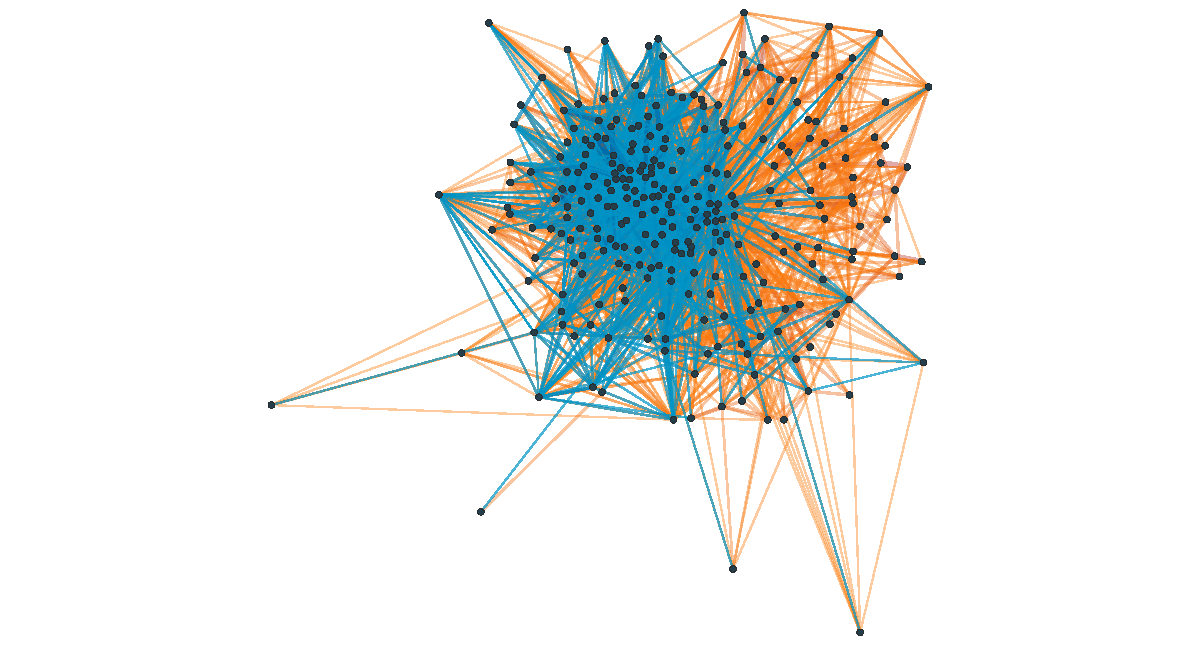
\includegraphics[width=15.0cm]{assets/connectome.pdf}}
\par\vspace{.15cm}
\textbf{\textit{C.~elegans}: 297 neurons, 3,604 chemical edges.} EleganSign [1].
\par
{\color{orange!80!black}Orange: positive}\quad {\color{blue!65!cyan}Blue: negative}\par
Largest connected component shown; arrows omitted.
\par\vspace{.2cm}
Fixed recurrent weights; only the readout is trained. Perturb topology, signs, and weights, then normalize spectral radius.
\par\vspace{.2cm}
\textbf{96 settings $\times$ 200 trials}\par
Vary target radius, leak rate, input scale, and bias.
\par\vspace{.2cm}
\textbf{IPC}: information processing capacity; nonlinear recall [2].\par
\textbf{KR}: kernel rank; history separation [3].\par
\textbf{MC}: memory capacity; recall of the past 30 inputs.
\par\vspace{.25cm}
$\displaystyle\mathrm{CV}=\frac{\mathrm{sd}}{\mathrm{mean}}$ across the 96 settings.\par\vspace{.2cm}
\textbf{Lower CV = greater robustness.}
}
\draw[rulecolor,line width=1pt] (20.5,-21) -- (20.5,-45.5);
\place{22}{20.8}{37}{\color{ink}\bodyfont
\heading{02\quad Performance comes with sensitivity}
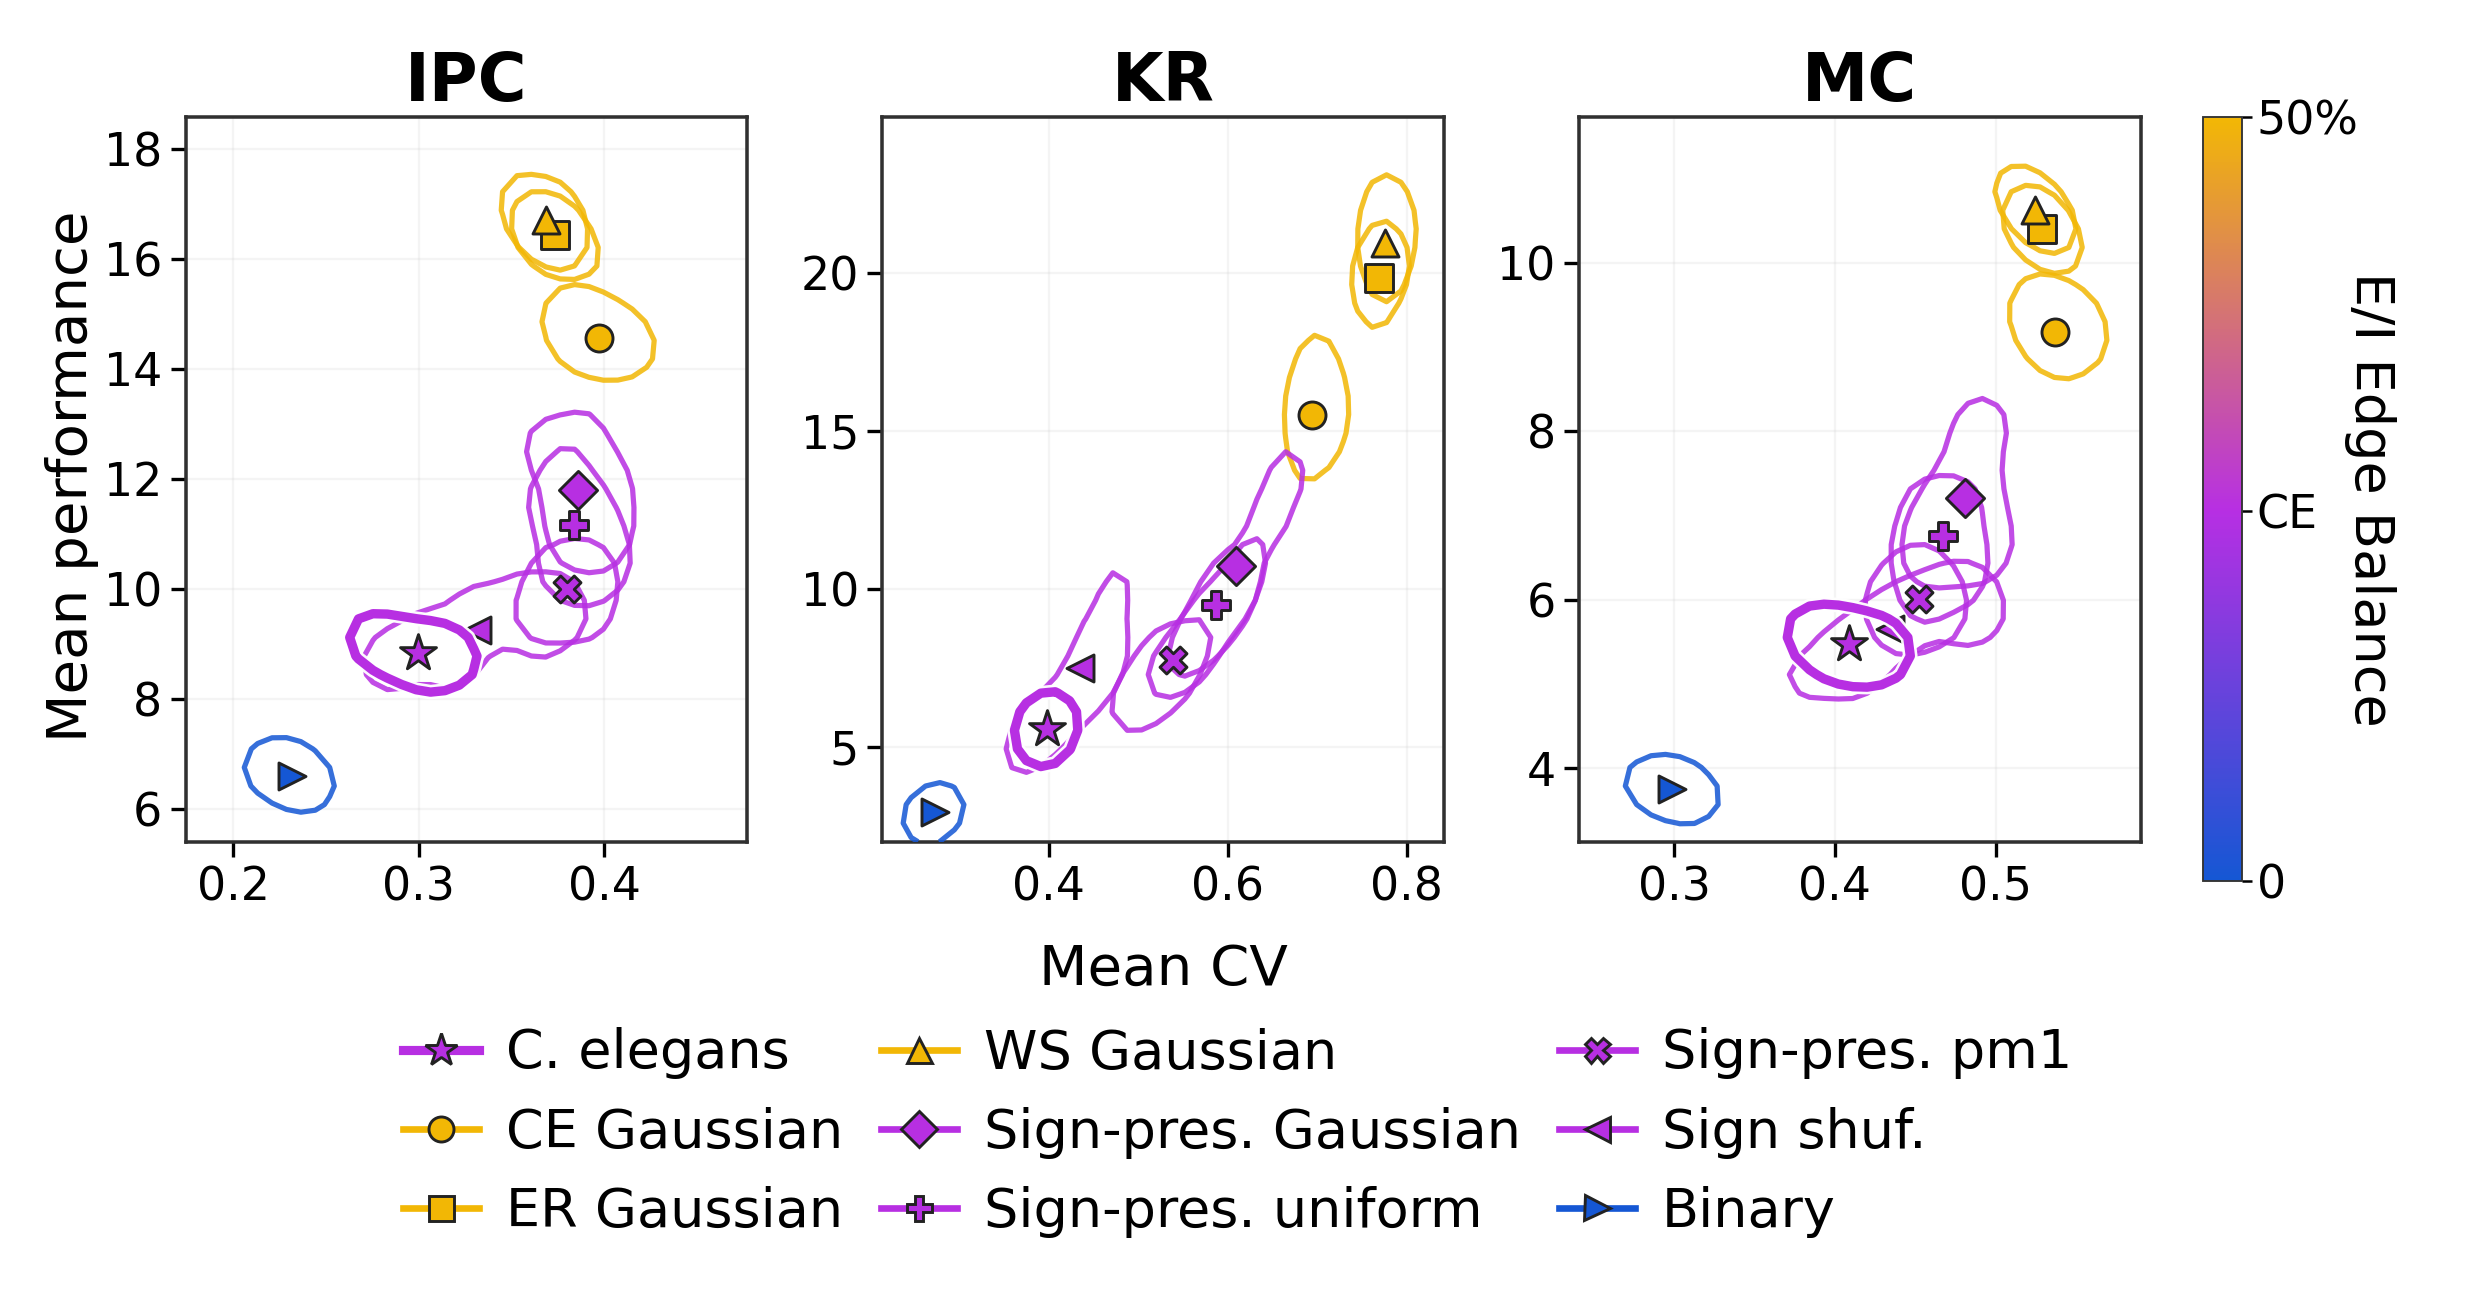
\includegraphics[width=37cm]{assets/architecture_tradeoff.png}
\vspace{.15cm}\par\smallfont
\textbf{Higher and farther right: more performance, less robustness.}
Mean performance: average across 96 settings. Contours enclose the highest-density 50\% of trials; markers identify architectures. Color indicates E/I edge balance: 0\%, CE $\approx24.25\%$, or 50\%.
\par
CE: \textit{C.~elegans}; ER: Erd\H{o}s--R\'enyi; WS: Watts--Strogatz. Sign-pres.: signs preserved; sign shuf.: signs shuffled; pm1: $\pm1$ weights.
}

\draw[rulecolor,line width=1pt] (2,-46.5) -- (59,-46.5);
\place{2}{47.5}{29}{\color{ink}\bodyfont
\heading{03\quad E/I balance traces the tradeoff}
\makebox[29cm][c]{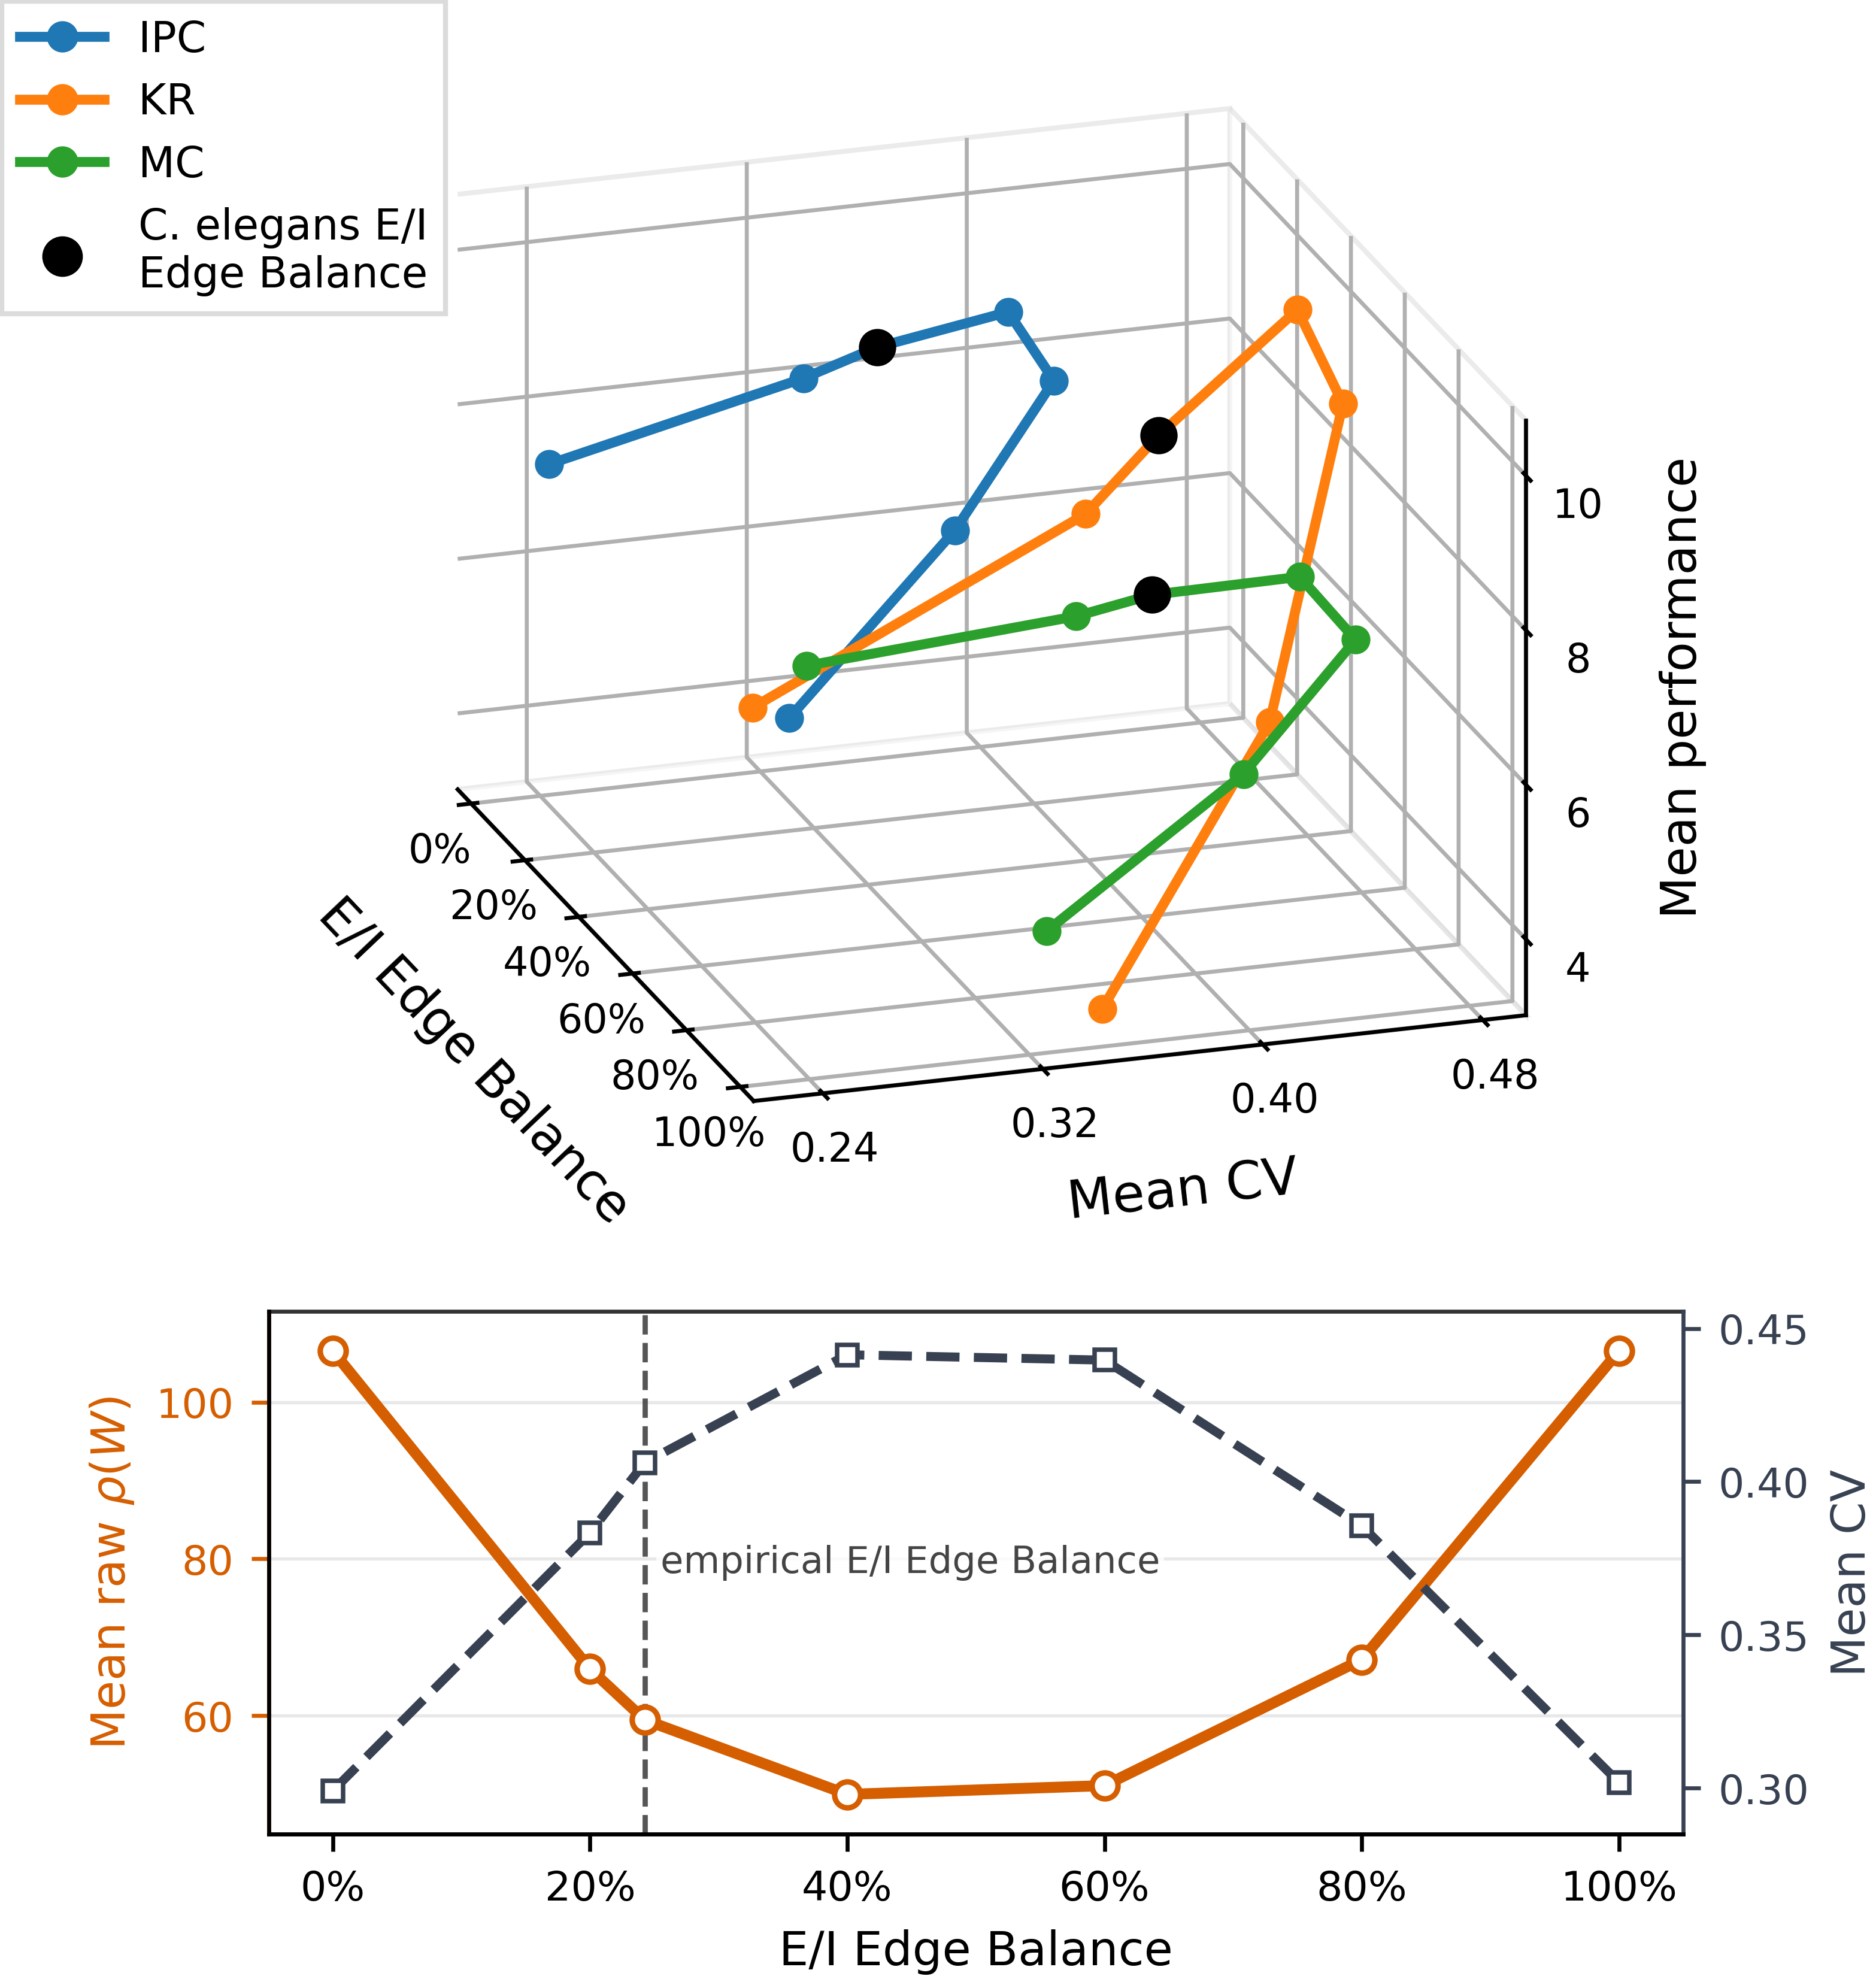
\includegraphics[width=23.0cm]{assets/performance_robustness_curves.png}}
\vspace{.3cm}\par\smallfont
\textbf{Changing signs moves performance and CV together.} Top: IPC, KR, and MC across E/I edge balance; black markers denote the empirical balance. Bottom: raw radius and CV averaged across metrics. Points average 200 trials.
}
\draw[rulecolor,line width=1pt] (32,-47.5) -- (32,-76.0);
\place{33}{47.5}{26}{\color{ink}\bodyfont
\heading{04\quad What the curves show}
Connectivity and weight magnitudes stay fixed while signs are randomly reassigned at each E/I edge balance.
\par\vspace{.5cm}
\textbf{Near the all-positive and all-negative endpoints:} lower performance and lower CV, indicating greater hyperparameter robustness.
\par\vspace{.5cm}
\textbf{Toward 50\% E/I edge balance:} higher performance and higher CV, indicating greater sensitivity to hyperparameter choice.
\par\vspace{.6cm}
\heading{Why normalization matters}
Every perturbed matrix $W'$ is rescaled:
\[
 W^{\mathrm{res}}=\frac{\rho_{\mathrm{target}}}{\rho_{\mathrm{raw}}}\,W',
 \qquad \rho_{\mathrm{raw}}=\max_i|\lambda_i(W')|.
\]
The raw radius decreases toward the balanced regime. Reaching the same target radius therefore requires a \textbf{larger scaling factor} in this regime.
\par\vspace{.5cm}
These curves combine changes in sign balance and placement with \textbf{normalization-induced rescaling}. They do not isolate a causal effect of E/I balance alone.
\par\vspace{.6cm}
{\color{teal}\fontsize{24}{29}\selectfont\bfseries Report raw spectral radius alongside architecture comparisons.}
\par\vspace{.5cm}
\smallfont The full paper finds the same qualitative tradeoff in an edge-matched random topology and after removing unknown or complex-sign edges.
}
\fill[pale] (2,-76.7) rectangle (59,-80.1);
\place{2.7}{77.15}{55.6}{\color{ink}\smallfont\textbf{Scope and limitations.} Robustness here means low relative variation across the tested hyperparameter grid; it does not imply invariance to all parameter changes. IPC omits products across different delays. Of 3,604 chemical edges, 1,864 have unknown or complex signs and are assigned signs to match the labeled-edge ratio; selected controls remove them. Electrical synapses and self-loops are excluded; input reaches all units.}
\place{2}{81}{57}{\color{muted}\fontsize{13}{17}\selectfont
\textbf{Selected references}\quad
[1] Fenyves et al. (2020). Synaptic polarity and sign-balance prediction. \textit{PLOS Comput. Biol.} 16, e1007974.\par
[2] Dambre et al. (2012). Information processing capacity of dynamical systems. \textit{Sci. Rep.} 2, 514.\par
[3] Roy \& Vetterli (2007). The effective rank: a measure of effective dimensionality. \textit{EUSIPCO}, 606--610.}
\end{scope}
\end{tikzpicture}
\end{document}
